\documentclass[12pt]{article}
\usepackage[english]{babel}
\usepackage[utf8x]{inputenc}
\usepackage[T1]{fontenc}
\usepackage{indentfirst}
\usepackage{scribe}
\usepackage{listings}
\usepackage{enumitem}

\Scribe{Group 23, Group 25, Group 26}
\Lecturer{Abir De}
\LectureNumber{12}
\LectureDate{26/09/2022}
\LectureTitle{Kernel Methods}

\lstset{style=mystyle}

%\newtheorem{theorem}{Theorem}[section]
\begin{document}
\MakeScribeTop



In this Lecture we discuss the smooth transition from Linear to Non-Linear space of functions. We discuss treatments where f(x) is non-linear in x that is, $f(x) \neq w^{T}x$, but we can construct it using our prior knowledge. We transform the data into a higher dimensional space and finds out that data is separable when transformed into higher dimensions.
We introduce "kernel method", a method of applying SVMs to problems with non linear classification boundaries. kernels are basically measure of similarity between two vectors.

\section{Introduction}
Remember we had a question in midsem (question 2.d) where the labels are +1 for all x such that |x| > 2 and −1 otherwise. We were asked to provide a 1D transformation $\phi : \mathbb{R} \rightarrow \mathbb{R}$  so that SVM applied to the given dataset. 
\begin{figure}[h]
\centering
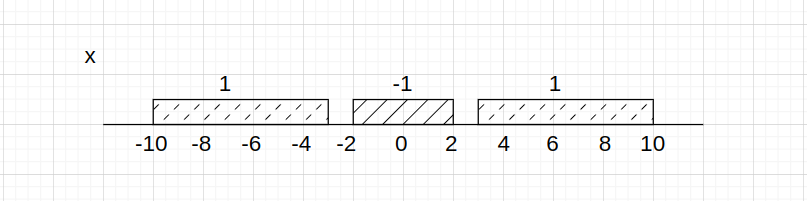
\includegraphics[width=0.9\linewidth]{input.png}
\caption{Initial input space : $x$} 
\end{figure} \newline
As it can be seen that SVM can not be applied to the initial input space. \\ 
Now let us first define a mapping $\phi\ :\ R \hookrightarrow R^2$ as follows:
\large{ 
\[
    \phi(x)\ =\ (x,x^2)
\]}
\begin{figure}[h]
\centering
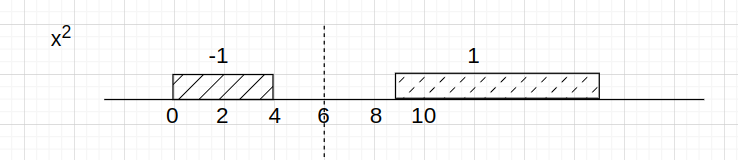
\includegraphics[width=0.9\linewidth]{transformed.png}
\caption{Transformed input space : $x^2$} 
\end{figure} 
Now our prediction will be $h(\phi(x))$ instead of $h(x)$, where $\phi(x) =x^2$ and $h$ is the learnt classifier, it is possible to apply SVM in the transformed space as seen in the Figure 2. \\

\noindent
\textbf{The Main Concept} behind Kernel Methods is that there is a possibility that, data-points that are not linearly-separable in lower dimensions are linearly-separable in higher dimensions. 


\section{Kernel Methods}
\noindent\textbf{The Basic Algorithm} will be:-
\vspace{-5pt}
\begin{itemize}
    \setlength\itemsep{2pt}
    \item Given some Data Set $S = (\{\bm{x_i}\}_{i=0}^n, \{y_i\}_{i=0}^n)$, where $\bm{x_i}\in \mathbb{R}^d$
    \item Consider a function $\bm{\phi}$ such that $\bm{\phi(x)} \in \mathbb{R}^{d'}$ where $d' > d$ (and can even be infinity)
    \item Create a new Data Set $\hat{S} = (\{\bm{\phi(x_i)}\}_{i=0}^n, \{y_i\}_{i=0}^n)$
    \item Train a linear Predictor $h$ over $\hat{S}$
    \item And then the prediction of any point $\bm{x_{test}}$ in the test dataset is given by $h(\bm{\phi(x_{test})})$
\end{itemize}
\noindent
Thus the prediction is given by $\bm{w^T\phi(x)}$ where both $\bm{w}, \bm{\phi(x)} \in \mathbb{R}^{d'}$ 

As $d'$ can reach infinity, this is theoretically possible for non linear functions but calculating and storing $\bm{w}$ and $\bm{\phi(x)}$ becomes practically impossible, but the dot product $\bm{w^T\phi(x)}$ is a scalar.

Here we are enriching the expressive power of halfspaces by first mapping the data into a high dimensional feature space, and then learning a linear predictor in that space. While this approach greatly extends the expressiveness of halfspace predictors, it raises both sample complexity and computational complexity challenges. We tackle this using the method of \textit{kernels}.

A popular choice for the mapping $\phi$ is a polynomial mapping: $x \rightarrow (1,x, x^2,\hdots)$ \\

\noindent
\textbf{The Setup:} \\Given a mapping $\phi$ we are left to solve the optimization problem:
\begin{align*}
    \min_w f(\{y_i\}_i^n , \{\bm{w^T\phi(x_i)}\}_i^n) + \lambda R(\bm{w})
\end{align*}
Where $f$ is a loss function and $R$ is a monotonic Regularization function.

\subsection{Transformation}
\begin{itemize}
    \item 
In a finite case if we sample $d$ dimension vector $N$ times such that $d << N$.
.It is with high probability that there will be $d$ vectors that are linearly independent of each other. But as the value of $d$ itself tends to infinity it becomes less and less likely

    \item
In the given case the vectors $\{\bm{\phi(x_i)}\}_i^n$ are of infinite dimension.
So if the optimum solution is $\bm{w^*}$ then there exists $\{\alpha_i\}_i^n$ such that $\bm{w^*}$ can be represented as 
\begin{align*}
    \bm{w^*} = \sum_{i = 0}^n \alpha_{i}*\bm{\phi(x_i)}\ + \bm{v}
\end{align*}
where $\bm{v^T\phi(x_i)} = 0$ for all $i$, that is, \textbf{v} is orthogonal to the span of the vectors mapped by the function $\phi$.

    \item
Let us define $\bm{w} = \bm{w^*} - \bm{v}$ 
\begin{align*}
    ||\bm{w}||^2 &= ||\bm{w^*} - \bm{v}||^2 \\
    ||\bm{w}||^2 &= ||\bm{w^*}||^2 - 2\bm{w^*}.\bm{v} + ||\bm{v}||^2 
    &\text{  As the value } \bm{w^*}.\bm{v} = \bm{v}.\bm{v} = ||\bm{v}||^2 \\
    ||\bm{w}||^2 &= ||\bm{w^*}||^2 - 2||\bm{v}||^2 + ||\bm{v}||^2 \\
    ||\bm{w}||^2 &= ||\bm{w^*}||^2 - ||\bm{v}||^2  
\end{align*}

    \item So as norm is a positive function we have $||\bm{w}|| \le ||\bm{w^*}||$
    \item And since $R$ is non-decreasing, we obtain $R(\bm{w}) \le R(\bm{w^*})$\\ ($R$ is monotonic regularization function as defined above)
    \item Also as $\bm{w^T\phi(x)} = (\bm{w^*} - \bm{v})^{\bm{T}}\bm{\phi(x)} = \bm{w^{*^T}\phi(x)}$ \\
    (since v is orthogonal to $\bm{\phi(x)}$, we have $\bm{v^T\phi(x)}$=0)
    \item And so,
\begin{align*}
    f(\{y_i\}_i^n , \{\bm{w^T\phi(x_i)}\}_i^n) = f(\{y_i\}_i^n , \{\bm{w^{*^T}\phi(x_i)}\}_i^n)
\end{align*}
    \item We have shown that the loss function is same for both $\bm{w^*}$ and $\bm{w}$ and the regularization function is less for $\bm{w}$ than $\bm{w^*}$,
    \item Hence  the objective function for $\bm{w}$ is less than that for $\bm{w^*}$, but as $\bm{w^*}$ is the optimum solution, we must have that $\bm{w}$ is also an optimum solution .

    \item Hence we have proved that the value 
    \begin{align*}
        \bm{w} = \sum_{i = 0}^n \alpha_i*\bm{\phi(x_i)}\
    \end{align*}
    is an optimum solution for the objective function.\footnote{Also remember that this was the result that we got by applying the Lagrange multiplier on the objective functions }
\end{itemize}

\begin{theorem} [\textbf{Representer Theorem}]
Given a mapping from $\mathbb{R}^d$ to $\mathbb{R}^{d'}$, there exists a vector 
$\bm{\alpha} \in \mathbb{R}^{d'}$ such that $\bm{w} = \sum_{i = 1}^{d'}\alpha_i \bm{\phi(x_i)}$ is an optimal solution.
\begin{align*}
    \min_w f(\{y_i\}_i^n , \{\bm{w^T\phi(x_i)}\}_i^n) + \lambda R(\bm{w})
\end{align*}     
\end{theorem}

\subsection{Kernel}
\noindent
Substituting the fact that $\bm{w} = \sum_{i = 1}^{d'}\alpha_i \bm{\phi(x_i)}$ is an optimum solution into the value $\bm{w^T\phi(x)}$
\begin{align*}
    \bm{w^T\phi(x)} &= \left( \sum_{i = 1}^{d'}\alpha_i \bm{\phi(x_i)^T} \right) \bm{\phi(x)} \\
        &= \sum_{i = 1}^{d'}\alpha_i \bm{\phi(x_i)^T\phi(x)} & \text{consider a function } K(\bm{x_i}, \bm{x_j}) = \bm{\phi(x_i)^T\phi(x_j)} \\
        &= \sum_{i = 1}^{d'}\alpha_i K(\bm{x_i}, \bm{x})
\end{align*}

Here $K$ is called a \textit{Kernel} Function and it denotes \textit{Similarity} between the data points $\bm{x_i}$ and $\bm{x_j}$. \\ \\
\noindent
What does this expression physically mean? We want to make a prediction at a new test point x, then $w^{*T} \phi(x)\ y(x)$ gives the \textbf{weighted mean} of labels $y(x_i)$ with weights as similarity 
$$ \mbox{ \large
$S(x,x_i)\ =\ \phi(x_i)^T \phi(x)$ 
} $$
thus giving more weight to similar neighbours. This essentially represents the idea of K-Means clustering. \\ 
We can note that this similarity function can be any form, not necessarily dot product, The term “kernels” is used in this context to describe inner product in the feature space  \\

\noindent
\large\textbf{Implications of this result}
\begin{itemize}[noitemsep,nolistsep]
    \item This representation takes us beyond SVM
    \item w is linear combination of $\phi(x_i)$ thus $w^T\phi(x)$ can be easily calculated. \\
\end{itemize}

\noindent
\textbf{Some Popular Kernels are:}
\begin{itemize}
    \item {\makebox[4cm][l]{\textbf{SVM}} &$K(\bm{x_i}, \bm{x_j}) = \bm{x_i^{T}x_j}$}
    \item {\makebox[4cm][l]{\textbf{Gaussian}} & $K(\bm{x_i}, \bm{x_j}) = e^{\frac{-||\bm{x_i} - \bm{x_j}||^2}{\sigma^2}}$}
    \vspace{3pt}
    \item {\makebox[4cm][l]{\textbf{k degree polynomial}} &$K(\bm{x_i}, \bm{x_j}) = (1 + \langle\bm{x_i}, \bm{x_j}\rangle)^k$}
\end{itemize}
where $\langle{.,.}\rangle$ denotes the inner product. \\ \\

\noindent
\textbf{\Large Exercise}\\
\textbf{\large{Que- Show that RBF can be written as inner product}}\\
It is easy to see that RBF(or Gaussian) Kernel satisfies the positive semidefinite condition, we can infact state and prove a possible inner product representation

Consider
\[
   \phi(x)\ =\ \sum_{n=0}^{\infty}  \frac{1}{\sqrt{n!}}e^{-\frac{x^2}{2}}x^n
\]

Observe that
{
\[ 
   <\phi(x),\phi(x^{'})>\ =\ \sum_{n=0}^{\infty}  \biggl( \frac{1}{\sqrt{n!}}e^{-\frac{x^2}{2}}x^n \biggl) 
   \biggl( \frac{1}{\sqrt{n!}}e^{-\frac{x^{'2}}{2}}x^{'n} \biggl)
\]
}
{ 
\[ 
   <\phi(x),\phi(x^{'})>\ =\  e^{-\frac{x^2 + x^{'2}}{2}} \sum_{n=0}^{\infty} \biggl( \frac{(xx^{'})^{n}}{n!} \biggl) 
\]
}
{ 
\[ 
   <\phi(x),\phi(x^{'})>\ =\  e^{-\frac{x^2 + x^{'2}}{2} + xx^{'}} 
\]
}
{
\[ 
   <\phi(x),\phi(x^{'})>\ =\  e^{-\frac{(x - x')^2}{2}} 
\]
}\\
\noindent
\textbf{{Que- Do the same for polynomial kernel}}\\
Left for reader\\
Hint: Solution can be checked in book Understanding machine learning chapter Kernel Methods

\section{SVM Kernel} \\
Now going back to the dual formulation of Hard-SVM:
\begin{align*}
   & \max_{\bm{\alpha}\in R^{D}:\bm{\alpha}\ge\bm{0}}(\sum_{i=1}^{D}\alpha_i - \frac{1}{2}\sum_{i=1}^{D}\sum_{j=1}^{D}\alpha_i\alpha_{j}y_{i}y_{j}\bm{x_i^{T}x_j}) \\
   &= \max_{\bm{\alpha}\in R^{D}:\bm{\alpha}\ge\bm{0}}(\sum_{i=1}^{D}\alpha_i - \frac{1}{2}\sum_{i=1}^{D}\sum_{j=1}^{D}\alpha_i\alpha_{j}y_{i}y_{j}K(\bm{x_i}, \bm{x_j}))\\
   &= \max_{\bm{\alpha}\in R^{D}:\bm{\alpha}\ge\bm{0}}(\sum_{i=1}^{D}\alpha_i - \frac{1}{2}\bm{(\alpha * Y)^{T}G{(Y*\alpha}}))        \\
   & \bm{*} \text{ denotes element-wise multiplication} \\
   & \bm{G} = \{K(\bm{x_i}, \bm{x_j})\}_{i,j=1}^{D \times D} \qquad\text{Known as the \textbf{Gram matrix}}
%^{DxD}   
\end{align*}
Hence, we are optimising for $\bm{\alpha}$ instead of $\bm{w}$. \\

The advantage of working with kernels rather than directly optimizing w in the feature space is that in some situations the dimension of the feature space is extremely large while implementing the kernel function is very simple.\\

\begin{theorem}[Mercers's Theorem]
$K : [ a,b] \times [ a,b] \rightarrow \mathbb{R}$ is a kernel if and only if :
\begin{enumerate} [nolistsep]
    \item Symmetric : $K(x,y) = K(y,x)$ for all $x,y \in [a,b]$, and
    \item Positive Semi-definite : $ \sum_{j=1}^{n} \sum_{j=1}^{n} K(x_i,x_j)c_i c_j \geq 0 $ for all finite sequences of points $\mathbf{x}_1, ..., \mathbf{x}_n$ of $[a, b]$ and all choices of real numbers $c_1, ..., c_n$
\end{enumerate}

\end{theorem}


\nocite{UNderstandingML}
\bibliographystyle{abbrv}          
\bibliography{mybib}                


\end{document}